\documentclass[12pt, a4paper]{article}
\usepackage[utf8]{inputenc}
\usepackage[czech]{babel}
\usepackage[T1]{fontenc}
\usepackage{graphicx}
\usepackage{amsmath, amssymb, amsthm}
\usepackage[margin=2.5cm]{geometry}
\usepackage{url}
\begin{document}

\begin{titlepage}
    \begin{center}
        {\large {Přírodovědecká fakulta}} \\
        \vspace{0.2cm}
        {\large Univerzita Karlova}
        
        \vspace{1.5cm}
        
\includegraphics[width=0.5\linewidth]{img/PrFUK_strom_digital_cerna.png} 
        \vfill{}
        
        {\huge\bfseries Konstrukce polyedrických globů} \\
        \vspace{0.5cm}
        {\large {Matematická kartografie}} \\
        \vfill
        
        \begin{center}
            \large Teodor Sorokáč \\
        \end{center}
        \vfill{}

        \begin{center}
            \ 2. N-GKDPZ \\
            \ Praha 2026
        \end{center}
        
    \end{center}
\end{titlepage}

\section{Zadání}

\vspace{5mm}
\subsection*{\textbf{Úloha č. 2: Konstrukce polyedrických globů}}

\vspace{3mm}
Vybraná platonská tělesa (šestistěn, čtyřstěn a osmistěn nebo dvanáctistěn) použijte pro polyedrickou aproximaci sféry. Na plošky platonských těles znázorněte v gnomické projekci geografickou síť doplněnou zákresem kontinentů. 
\vspace{3mm}

\[
\begin{aligned}
x &= R \cdot \tan(90^\circ - \text{š}) \cos d, \\
y &= R \cdot \tan(90^\circ - \text{š}) \sin d,
\end{aligned}
\]

\noindent Skript pro generování sítě poledníků, rovnoběžek a znázornění kontinentů realizujte v programu MATLAB bez použití extreních funkcí. Soubory se zákresem kontinentů exportujte z vhodné datové sady.
\vspace{3mm}

\noindent Vytvořte prostorové modely polyedrických globů v měřítku 1:100 000 000 nebo 1:50 000 000 dle možnosti Vaší tiskárny a pošlete fotografii/video Vašeho glóbu. Součástí úlohy bude příloha s rozloženými modely globů.
\vspace{3mm}

\noindent Zjistěte následující vlastnosti gnomonické projekce v~okrajovém bodě~$Q$ jedné ze~stěn Platonského tělesa:
\begin{itemize}
    \item měřítko $m_p$ v poledníku, měřítko $m_r$ v rovnoběžce,
    \item poloosy $a$, $b$ Tissotovy indikatrix,
    \item úhel $\omega^\prime$ mezi obrazem poledníku a rovnoběžky,
    \item maximální úhlové zkreslení $\Delta \omega$,
    \item měřítko ploch $P$
\end{itemize}

\noindent Vypočtené parametry v bodě $Q$ použijte k zákresu Tissotovy indikatrix (doporučené měřítko 1:1 000 000), jako podklad využijte obraz geografické sítě na příslušné stěně Platonského tělesa v gnomonické projekci, volte $\Delta u = \Delta v = 10^\circ$ (formát A4, popř. odpovídající).
\vspace{3mm}

\noindent Výpočty proveďte pro referenční kouli s poloměrem $R = 6380$ km, hodnoty měřítek a~poloos Tissotovy indikatrix uveďte s přesností na 6 desetinných míst, úhlové hodnoty s přesností na $^{\prime\prime}$. Výsledky zkontrolujte s hodnotami získanými z programu Proj.4. 

\vspace{1cm}
\subsection*{\textbf{Hodnocení:}}

\begin{center}
\resizebox{\textwidth}{!}{
\begin{tabular}{|l|c|}
\hline
\textbf{Krok}                                                                                  & \textbf{Hodnocení} \\ [0.5ex]  \hline\hline
\rule{0pt}{3ex} Konstrukce polyedrických globů (4- a 8- nebo 12- stěn).                                    &  20b              \\ \hline
\rule{0pt}{3ex}\textit{Konstrukce polyedrického globu (20- stěn)}                    & \textit{+10b}    \\ \hline
\rule{0pt}{3ex}\textit{Digitální 3D model globu.} & \textit{+10b}    \\ \hline
\rule{0pt}{3ex}\textit{Mapa na povrchu globu.}   & \textit{+5b}    \\ \hline
\rule{0pt}{3ex}\textit{Skript v Pythonu pro tvorbu 3D modelu s mapou na povrchu.} & \textit{+20b} \\ \hline
\rule{0pt}{3ex}\textit{Výpočet meridiánové konvergence.}                    & \textit{+5b}    \\ \hline
\rule{0pt}{3ex}\textit{Kontrola zkreslení v knihovně \textit{Proj.4.}}                    & \textit{+15b}    \\ \hline
\rule{0pt}{3ex}\textit{Prostorový model na 3D tiskárně měřítku 1:100 000 000 nebo 1:50 000 000}                    & \textit{+10b}    \\ \hline
\rule{0pt}{3ex}\textbf{Max celkem:} & \textbf{95b} \\ \hline
\end{tabular}
}
\end{center}
\vspace{5mm}

\subsection*{Řešené bonusové úlohy}
V rámci úlohy byly vypracované následující bonusové úlohy: \textit {Mapa na povrchu (5b), Výpočet meridiánové konvergence. (5b), Kontrola zkreslení v knihovně \textit{Proj.4.} (15b)}

\newpage
\section{Popis a rozbor problému}
\vspace{5mm}
Polyedrické globy jsou specifickou aproximací sférického povrchu pomocí tělesa s rovinnými stěnami. Cílem této úlohy je vytvoření modelu polyedrického globu. Převod zeměpisných souřadnic je zajištěn gnomonickou projekcí, která je pro tuto úlohu ideální, protože zobrazuje hlavní kružnice (ortodromy) jako úsečky. To je klíčové pro sestavení polyedrického globu, v mém případě dvanáctistěnu, bez překryvů a spár.
\vspace{3mm}

\noindent Pro veškeré výpočty bylo využito prostředí MATLAB. Bylo vytvořeno několik skriptů a funkcí, které nejprve určí geometrii zvoleného tělesa. Následně je pro každou stěnu vygenerována geografická síť a jsou transformovány obrazy kontinentů. Součástí je také výpočet Tissotovy indikatrix, konkrétně jejích poloos a měřítek v poledníku a rovnoběžce. Pro ověření správnosti analytických výsledků bylo využito externí knihovny Proj.4.

\subsection*{Gnomonická projekce}
\noindent Pro převod zeměpisných souřadnic do kartografických byla použita gnomonická projekce. Jedná se o azimutální zobrazení, kde střed promítání leží v těžišti referenční koule. Zobrazovací rovnice gnomonické projekce v obecné poloze jsou:
\vspace{3mm}

$$x = R \cdot \tan(90^{\circ} - s) \cos d$$
\vspace{3mm}
$$y = R \cdot \tan(90^{\circ} - s) \sin d$$
\vspace{3mm}

\noindent Parametry $s$ a $d$ jsou transformované souřadnice a $R$ je zemský poloměr ($R = 6380$ km). Poledníky se v normální poloze zobrazují jako polopřímky a rovnoběžky jako soustředné kružnice.

\newpage
\subsection*{Pravidelný dvanáctistěn}
Pravidelný dvanáctistěn je tvořen 12 pravidelnými pětiúhelníky. Těžiště pětiúhelníků odpovídají kartografickým pólům pro jednotlivé plošky. Na základě geometrie byla odvozena zeměpisná šířka pólů na severní polokouli ($\alpha_n$):
$$u_{\alpha} = \alpha_n \approx 26.5651^{\circ}$$

\noindent Kartografické póly na severní polokouli ($K_1$ až $K_5$) mají souřadnice:
$$K_1=[u_{\alpha}, 0^{\circ}], K_2=[u_{\alpha}, 72^{\circ}], K_3=[u_{\alpha}, 144^{\circ}], K_4=[u_{\alpha}, 216^{\circ}], K_5=[u_{\alpha}, 288^{\circ}]$$

\noindent Díky středové souměrnosti mají kartografické póly na jižní polokouli ($K_6$ až $K_{10}$) zeměpisnou šířku s opačným znaménkem $\alpha_s = -26.5651^{\circ}$:
$$K_6=[-\alpha_n, 36^{\circ}], K_7=[-\alpha_n, 108^{\circ}], K_8=[-\alpha_n, 180^{\circ}], K_9=[-\alpha_n, 252^{\circ}], K_{10}=[-\alpha_n, 324^{\circ}]$$

\noindent Zbylé dva póly odpovídají severnímu a jižnímu pólu ($K_{11}=[90^{\circ}, 0^{\circ}]$, $K_{12}=[-90^{\circ}, 0^{\circ}]$). 
\vspace{3mm}

\noindent Pro oříznutí plošek je nutné definovat okrajové body. Jejich zeměpisné šířky jsou určeny doplňkovými úhly $\gamma_n$ a $\delta_n$:
$$u_{\gamma} = \gamma_n \approx 52.6226^{\circ}$$
$$u_{\delta} = \delta_n \approx 10.8123^{\circ}$$

\noindent Pro jižní polokouli platí hodnoty s opačným znaménkem ($\gamma_s = -52.6226^{\circ}$ a $\delta_s = -10.8123^{\circ}$).
\vspace{3mm}

\noindent Na základě těchto úhlů a zeměpisných délek byly ve skriptech \textit{u2\_north.m} a \textit{u2\_south.m} definovány hranice pro všech 12 plošek.

\newpage
\section{Výpočty a mezivýpočty}
Pro zhodnocení kvality zobrazení na okraji plošky (okrajový bod stěny $Q$ ležící ve středu její hrany) bylo nutné vypočítat základní charakteristiky zkreslení.
\vspace{3mm}

\noindent Měřítko v poledníku $m_p$ se počítá jako $m_p = 1 / \cos^2 \psi$.
\vspace{3mm}

\noindent Měřítko v rovnoběžce $m_r$ se počítá se jako $m_r = 1 / \cos \psi$, kde $\psi$ je sférická vzdálenost bodu od středu plošky. 
\vspace{3mm}

\noindent U azimutálních zobrazení tyto hodnoty přímo odpovídají hlavním poloosám Tissotovy indikatrix, platí tedy $a = m_p$ a $b = m_r$. Měřítko ploch $P$ je součinem obou poloos ($P = a \cdot b$).
\vspace{3mm}

\noindent Maximální úhlové zkreslení $\Delta \omega$ se určí ze vztahu:
$$\sin \left( \frac{\Delta \omega}{2} \right) = \frac{a - b}{a + b}$$
\vspace{3mm}

\noindent Meridiánová konvergence udává úhel, který svírá obraz místního poledníku s osou y.

\subsection*{Skripty v programech}
\vspace{5mm}
Všechny skripty pro tvorbu polyedrického globu a výpočty zkreslení byly realizovány ve vlastních funkcích v prostředí MATLAB:
\begin{itemize}
    \item \textit{gnom.m} -- funkce pro výpočet gnomonické projekce.
    \item \textit{uvTosd.m} -- funkce pro transformaci zeměpisných souřadnic.
    \item \textit{graticule.m} -- funkce pro vykreslení geografické sítě (poledníky a rovnoběžky).
    \item \textit{continent.m} -- funkce pro nahrání a transformaci kontinentů.
    \item \textit{GlobeFace.m} -- funkce pro vykreslení jedné kompletní stěny.
    \item \textit{gnom\_distortions.m} -- funkce pro výpočet derivací a vykreslení Tissotovy indikatrix pro okrajový bod.
    \item \textit{u2\_north.m} / \textit{u2\_south.m} -- skripty zajišťující vykreslení všech 12 stěn.
\end{itemize}

\newpage
\subsection*{Konstrukce polyedrického globu}
\vspace{5mm}
Prvním krokem konstrukce bylo definování společných parametrů (krok sítě $10^\circ$, měřítko a referenční poloměr). Následně byly definovány hraniční body a středy pro každou z 12 plošek. Geografická síť i souřadnice lomových bodů kontinentů byly transformovány ke středům ploch. Výstupy byly oříznuty na přesný tvar pravidelného pětiúhelníku, aby nedošlo k špatnému sestavení modelu a plochy na sebe navazovaly.
\vspace{10mm}


\begin{figure}[h]
\centering
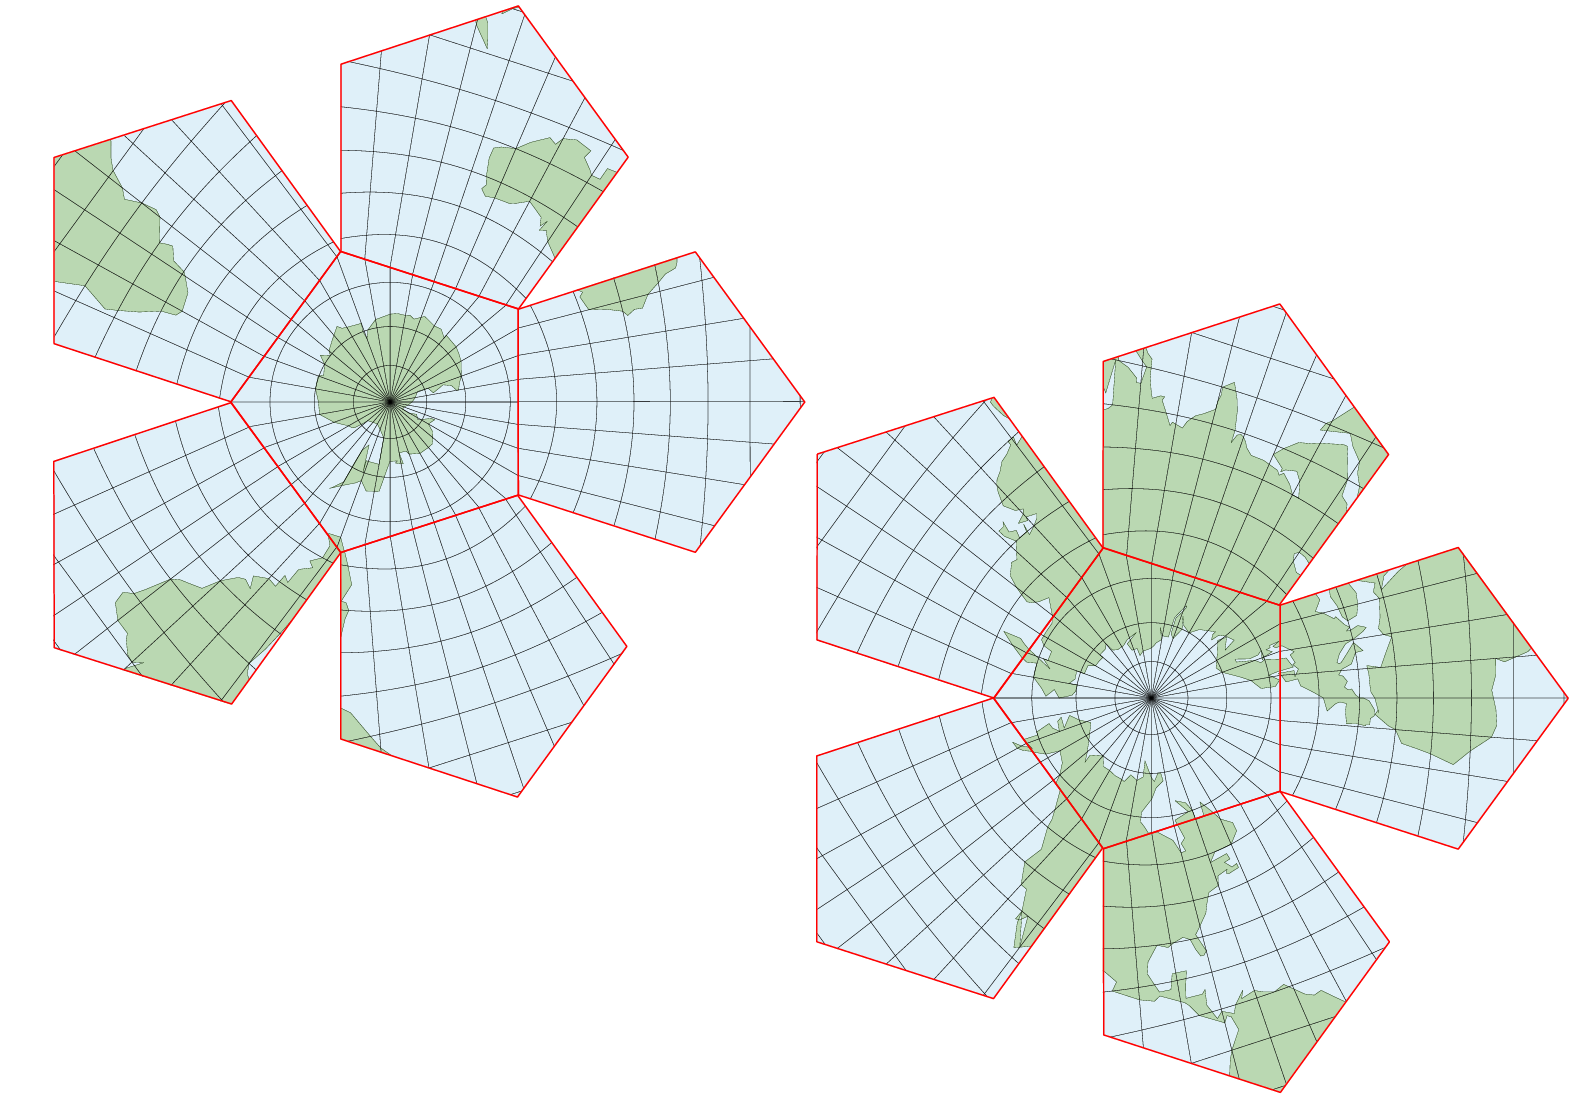
\includegraphics[width=1\textwidth]{img/12sten.png}
\caption{Rozložené plošky polyedrického globu vygenerované v MATLABu}
\end{figure}

\newpage
\section{Kontrola zkreslení pomocí knihovny Proj.4}
\vspace{5mm}
Pro ověření správnosti výpočtů z prostředí MATLAB byla provedena kontrola pomocí kartografické knihovny Proj.4 (v implementaci pro Python \textit{pyproj}). Pro porovnání bylo nastaveno sférická koule s poloměrem $R = 6380$ km a gnomonická projekce.
\vspace{3mm}

\noindent Pro zvolený bod $Q = [58{,}282526^\circ; 72^\circ]$ byly vygenerovány hodnoty délkových měřítek a úhlových zkreslení. Tyto hodnoty byly následně porovnány s výsledky z MATLABu, jak shrnuje Tabulka 1.

\begin{table}[h]
\centering
\renewcommand{\arraystretch}{1.2}
\begin{tabular}{|l|c|c|}
\hline
\textbf{Vlastnosti gnomonické projekce v bodě $Q$} & \textbf{Hodnota (MATLAB)} & \textbf{Hodnota (Proj.4)} \\ \hline
Měřítko v poledníku $m_p$ & $1.381966$ & $1.381966$ \\ \hline
Měřítko v rovnoběžce $m_r$ & $1.175570$ & $1.175570$ \\ \hline
Poloosa $a$ Tissotovy indikatrix & $1.381966$ & $1.381966$ \\ \hline
Poloosa $b$ Tissotovy indikatrix & $1.175570$ & $1.175570$ \\ \hline
Úhel $\omega^\prime$ mezi poledníkem a rovnoběžkou & $90^{\circ}$ & $90^{\circ}$ \\ \hline
Maximální úhlové zkreslení $\Delta\omega$ & $9^\circ 15^\prime 28^{\prime\prime}$ & $9^\circ 15^\prime 28^{\prime\prime}$ \\ \hline
Měřítko ploch $P$ & $1.624598$ & $1.624598$ \\ \hline
Meridiánová konvergence $c$ & $18^{\circ}$ & $72^{\circ}$ \\ \hline
\end{tabular}
\caption{Porovnání vlastností gnomonické projekce ve středu hrany plošky}
\end{table}

\noindent Z porovnání výsledků obou postupů je patrné, že došlo ke správnému sestavení zobrazovacích rovnic, protože hodnoty měřítek a zkreslení se shodují. Jediný znatelný rozdíl nastal u meridiánové konvergence.

\begin{figure}[h]
\centering
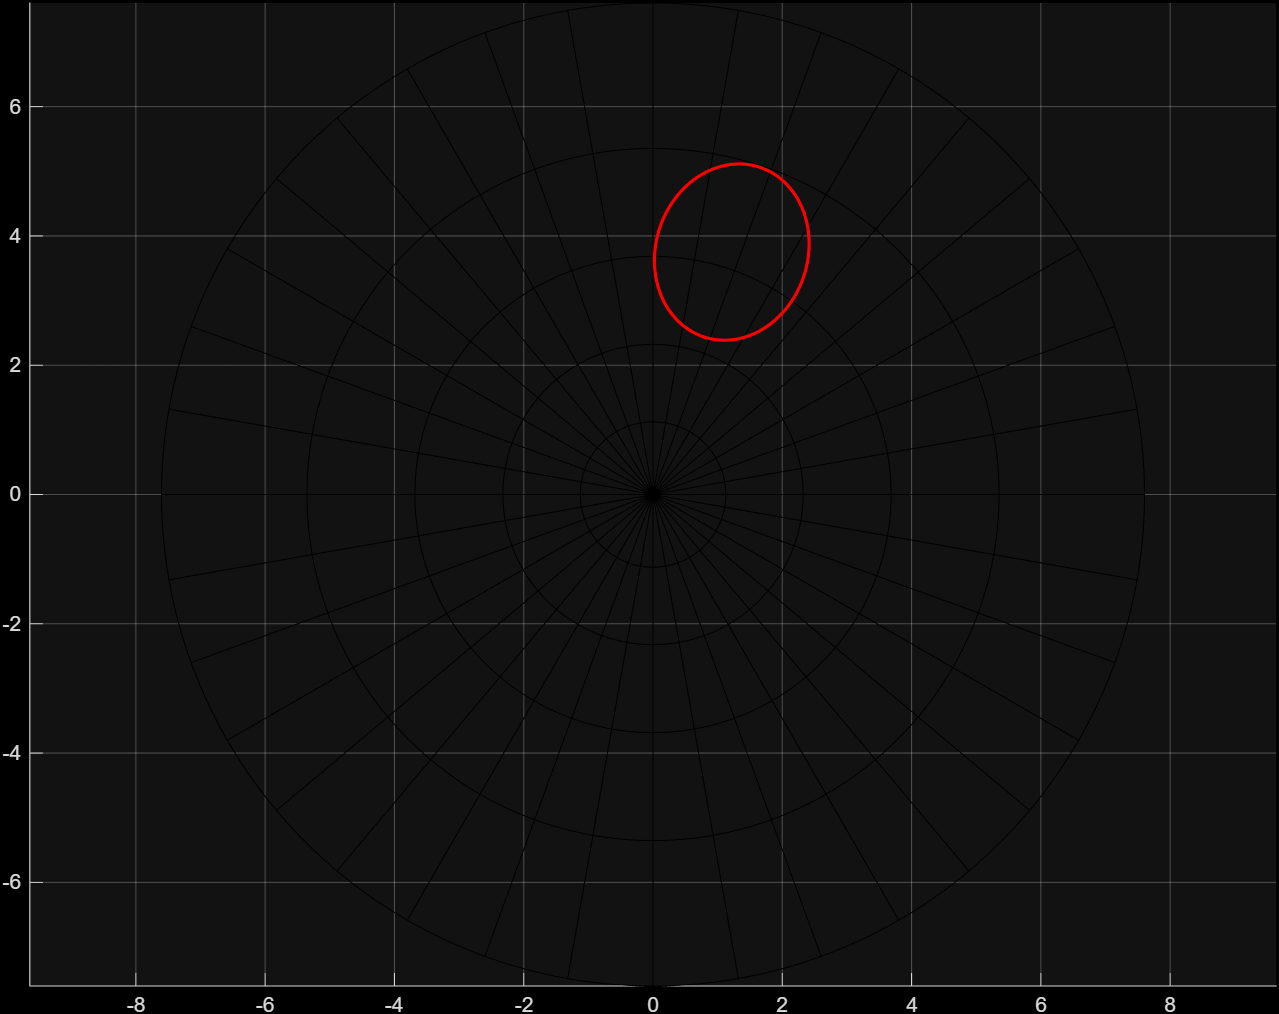
\includegraphics[width=0.6\textwidth]{img/tiss_indx.png}
\caption{Tissotova indikatrix}
\end{figure}

\newpage
\section{Zhodnocení výsledků a závěr}
\vspace{5mm}
Cílem úlohy bylo vytvoření modelu polyedrického globu, za pomoci vypočetního programu MATLAB. Cíl úlohy byl splněn a kontrola pomocí knihovny pyproj ověřila správnost výsledků. 
\vspace{3mm}

\noindent Z provedené analýzy v testovaném okrajovém bodě (ve středu hrany plošky) vyplývá, že gnomonická projekce v těchto místech deformuje plochy, které se oproti realitě zvětšují přibližně 1,6krát ($P \approx 1.62$). Délkové měřítko se zde protahuje více ve směru poledníků ($m_p$) než ve směru rovnoběžek ($m_r$).

\newpage
\section{Seznam literatury}
\vspace{5mm}
BAYER, T. (2026): Kartografická zkreslení. Délkové zkreslení, plošné zkreslení, podmínky konformity. Tissotova indikatrix. Přednáška pro předmět Matematická kartografie, Katedra aplikované geoinformatiky a kartografie, Přírodovědecká fakulta UK [cit. 31. 5. 2026].
\vspace{3mm}

\noindent BAYER, T. (2026): Konstrukce globů na platonských tělesech - návod na cvičení. Výukový materiál pro předmět Matematická kartografie, Katedra aplikované geoinformatiky a kartografie, Přírodovědecká fakulta UK [cit. 31. 5. 2026].

\end{document}
